%% Los cap'itulos inician con \chapter{T'itulo}, estos aparecen numerados y
%% se incluyen en el 'indice general.
%%
%% Recuerda que aqu'i ya puedes escribir acentos como: 'a, 'e, 'i, etc.
%% La letra n con tilde es: 'n.

\chapter{Métodos}
%\setcounter{section}{1}
\section{Métodos estadísticos}

\subsection{Modelo AMMI y SREG}

El modelo AMMI propuesto por Zobel et al. (1988) es un modelo multiplicativo en el cual se expresa el fenotipo de un genotipo en un ambiente de la siguiente forma:
\begin{center}
$y_{ij}= \mu +G_i + A_j + \sum_{k=1}^q \lambda_k \alpha_{ik} \gamma_{jk}$ \hspace{0.5cm} $ i=1,...,g$;\hspace{0.15cm} $ j=1,...,a$;\hspace{0.15cm} $q=min(g-1,a-1)$
\end{center} 
donde 
\begin{itemize}
\item $y_{ij}$ es el caracter fenotípico evaluado (rendimiento o cualquier otro caracter de interes) del $i$-ésimo genotipo en el $j$-ésimo ambiente,
\item $\mu$ es la media general,
\item  $G_i$ es el efecto del $i$-ésimo genotipo,
\item $A_j$ es el efecto del $j$-ésimo ambiente
\item $\sum_{k=1}^q \lambda_k \alpha_{ik} \gamma_{jk}$ es la sumatoria de componentes multiplicativas utilizadas para modelar la IGA. Siendo, $\lambda_k$ el valor singular para la  $k$-ésima componente principal (PC) $\alpha_{ik}$ y $\gamma_{jk}$ son los scores de las PC para el $i$-ésimo genotipo y el $j$-ésima ambiente para la $k$-ésima componente, respectivamente;
\end{itemize}

En cambio, el modelo SREG (Cornelius et al., 1996; Crossa y Cornelius, 1997 y 2002) expresa el fenotipo de un genotipo en un ambiente en función del efecto ambiente aditivo y los efectos genotipo e interacción agrupados y en forma multiplicativa:
\begin{center}
$y_{ij}= \mu +  A_j + \sum_{k=1}^q \lambda_k \alpha_{ik} \gamma_{jk}$ \hspace{0.5cm} $ i=1,...,g$;\hspace{0.15cm} $ j=1,...,a$; \hspace{0.15cm} $q=min(g-1,a-1)$
\end{center} 

Los parámetros multiplicativos, tanto en el modelo AMMI como en el SREG, se estiman por medio de la DVS de la matriz que contiene los residuos del modelo aditivo luego de ajustar por mínimos cuadrados el modelo de efectos principales. Generalmente los dos primeros términos multiplicativos son suficientes para explicar los patrones de interacción; la variabilidad remanente se interpreta como ruido. 

Para visualizar el efecto de IGA o conjuntamente el efecto de G y IGA se proponen los gráficos biplots GE y GGE (proveniente de las siglas en inglés G de Genotipe y GE de Genotipe-Environment) (Yan et al., 2000) respectivamente. El concepto del biplot fue presentado por Gabriel (1971), que consiste en una representación de las filas (individuos) y las columnas (variables) de una matriz de datos en un mismo gráfico. Éstos biplots, son herramientas poderosas definidas para el análisis e interpretación de la estructura de datos provenientes de ensayos multiambientales utilizados en los programas de mejoramiento (Ebdon y Gauch, 2002; Samonte et al., 2004; Yan et al., 2000; Zobel et al., 1988).

El biplot GE ayuda a interpretar la variación producida por los efectos de la IGA. Por otro lado, el biplot GGE permite investigar la diferenciación de mega-ambientes entre los ambientes en estudio, seleccionar cultivares superiores en un mega-ambiente dado y seleccionar los mejores ambientes de evaluación para analizar las causas de la interacción GA. Se define como mega-ambiente a un grupo de ambientes en donde los cultivares de mejor desempeño son los mismos.


\subsection{Modelo AMMI robusto}

El modelo AMMI, en su forma estándar, asume que no hay valores atípicos en el conjunto de datos. La presencia de observaciones atípicas es más una regla que una excepción cuando se consideran datos agronómicos debido a errores de medición, algunas plagas / enfermedad que puede influir en algunos genotipos  resultando por ejemplo en un rendimiento inferior al esperado en un ambiente, o incluso debido a alguna característica inherente de los genotipos que se evalúan.

Rodrigues et al. (2015) proponen una generalización robusta del modelo AMMI, que se puede obtener en dos etapas: primero ajustar la regresión robusta basada en el estimador M-Huber (Huber, 1981) para reemplazar el ANOVA; y luego utilizar un procedimiento DVS / PCA robusto para reemplazar la DVS estándar. En la segunda etapa, consideraron varios métodos dando lugar a total de cinco modelos robustos llamados: R-AMMI, H-AMMI, G-AMMI, L-AMMI, PP-AMMI. 

El empleo de la versión robusta del modelo AMMI puede ser extremadamente útil debido a que una mala representación de genotipos y ambientes en los biplots puede dar como resultado un mala decisión con respecto a qué genotipos seleccionar para un conjunto dado de ambientes (Gauch1997,Yanetal2000). A su vez, la elección de los genotipos incorrectos pueden provocar grandes pérdidas en términos de producción de rendimiento. Los biplots obtenidos de los modelos robustos mantienen las características e interpretación estándar del modelo AMMI clásico (Rodrigues et al. (2015)).


\subsection{Métodos de imputación}


Una limitación importante que presentan los modelos multiplicativos descriptos previamente es que requieren que el conjunto de datos este completo, es decir no admiten valores perdidos. Aunque los EMA están diseñados para que todos los genotipos se evalúen en todos los ambientes, la presencia de valores faltantes es muy común debido a errores de medición o pérdidas de plantas por animales, inundaciones o problemas durante la cosecha, además de la dinámica propia de la evaluaciones en las que se incorporan y se descartan genotipos debido a su pobre desempeño (Hill y Rosemberg, 1985)

Se han propuesto numerosas metodologías para superar el problema de valores ausentes en el conjunto de datos, entre las cuales se encuentran:

\begin{itemize}
\item EM-AMMI: Gauch y Zobel (1990) desarrollaron un procedimiento iterativo que utiliza el algoritmo de maximización de la esperanza (EM, del inglés \emph{Expectation-Maximization}) incorporando el modelo AMMI. \textbf{Este método reemplaza... (poner como abajo)}. Dependiendo del número de términos multiplicativos empleados, el método de imputación puede denominarse EM-AMMI0, EM-AMMI1, etc. (Gauch y Zobel 1990). 
\end{itemize}
\begin{itemize}
\item EM-SVD: Perry (2009a) propone un método de imputación que combina el algoritmo EM con DVS. Este método, en forma similar al anterior, reemplaza los valores faltantes de una matriz $G \times E$ inicialmente por valores arbitrarios para obtener una matriz completa, y luego la DVS se calcula iterativamente en esa matriz. 
\end{itemize}
\begin{itemize}
\item EM-PCA:
\end{itemize}
\begin{itemize}
\item Gabriel Eigen: Arciniegas-Alarcón et al. (2010) propuso un método de imputación que combina regresión y aproximación de rango inferior usando DVS. El método reemplaza inicialmente las celdas faltantes por valores arbitrarios, y posteriormente el
las imputaciones se refinan a través de un esquema iterativo que define una partición de la matriz para cada valor que falta a su vez y utiliza una regresión lineal de columnas (o filas) para obtener el nueva imputación. En esta regresión, la matriz de diseño se aproxima por una matriz de menor rango usando la DVS.
\end{itemize}
\begin{itemize}
\item WGabriel Eigen:
\end{itemize}




\section{Paquete de R}

%https://oscarperpinan.github.io/R/Paquetes.html 
En R, la unidad fundamental de código que se puede compartir es el paquete. Éste agrupa códigos, datos, documentación y pruebas, y es fácil de compartir con otros. Para crear uno de ellos, se deben seguir los siguientes pasos:

\begin{itemize}
\item Crear el paquete.
\item Crear, modificar y probar archivos .R
\item Verificar 
\item Redacción de la documentación.
\item Verificar 
\item Instalar.
\end{itemize}

Para el desarrollo del paquete se utilizan numerosas funciones incluidas en el paquete \emph{devtools} \citep{Hadley2019} ya que facilita el proceso de creación del mismo. Antes de comenzar, se debe tener instalada la última versión de R, luego mediante el siguiente código se instalarán los paquetes que se necesitan:

\begin{lstlisting}
install.packages(c("devtools", "roxygen2", "testthat", "knitr"))
\end{lstlisting}

Se debe contar ademas con una versión reciente del IDE de RStudio. 

\subsection{Creación del paquete}

Para crear la estructura del paquete se utiliza la función \textcolor{blue}{create\_package}(). El principal y único argumento requerido por dicha función es el directorio donde el nuevo paquete se alojará. Por lo general, si el directorio se llama ``geneticae'', entonces el nombre del paquete también será ``geneticae'':


\begin{lstlisting}
# Cargar la libreria devtools
library(devtools)
# Crear el paquete geneticae
create_package(``C:/Users/Julia/Desktop/geneticae")
\end{lstlisting}


El resultado de ejecutar la función \textcolor{blue}{create\_package}() es un paquete con los siguientes componentes:
\begin{itemize}
\item Un directorio R/.
\end{itemize}
\begin{itemize}
\item DESCRIPTION, un archivo simple cuyo objetivo es almacenar metadatos importantes sobre el paquete, epecifica el título, la versión del mismo, identifica al autor y brinda un mail de contacto, una breve descripción del paquete, la lista de los paquetes que el paquete creado necesita para funcionar, la licencia, entre otros.

El contenido básico en un archivo DESCRIPTION es:
\end{itemize}

\begin{verbatim}
Package: geneticae
Title: What the Package Does (One Line, Title Case)
Version: 0.0.0.9000
Authors@R: 
    person(given = "First",
           family = "Last",
           role = c("aut", "cre"),
           email = "first.last@example.com",
           comment = c(ORCID = "YOUR-ORCID-ID"))
Description: What the package does (one paragraph).
License: What license it uses
Encoding: UTF-8
LazyData: true
\end{verbatim}




\begin{itemize}
\item Un archivo NAMESPACE
\end{itemize}

Estas carpetas se iran modificando a medida que el paquete se vaya creando. También puede incluir un archivo de proyecto de RStudio pkgname.Rproj, que hace que el paquete sea fácil de usar con RStudio; .Rbuildignore enumera los archivos que se necesitan, pero que no deben incluirse al compilar el paquete R desde la fuente; .gitignore anticipa el uso de Git.
Se crearán, a través de devtools, las siguientes carpetas: data/ y  man/.




\subsection{Creación de funciones y conjuntos de datos}

Una vez creada la estructura del paquete se deben incluir las funciones que el mismo contendrá. Cada una de ellas debe ser guardada en un archivo de extensión .R, en el subdirectorio R/. Para ello, se utiliza la función \textcolor{blue}{use\_r}() la cual crea y/o abre un script de la carpeta R/.

Una vez creada una función, se realizan pruebas para asegurar que el código realice lo que realmente se desea utilizando la función \textcolor{blue}{load\_all}() que simula el proceso de construcción, instalación y conexión del paquete. Permite que las funciones creadas estén disponible rápidamente para uso interactivo, del mismo modo que si se hubiera construido e instalado el paquete y luego cargada en la sesión de R a través de la función \textcolor{blue}{library}(geneticae).

Muy frecuentemente se utilizan funciones que se encuentran disponibles en otros paquetes, para ello se utiliza la función \textcolor{blue}{use\_package}() que agrega el paquete al archivo DESCRIPTION.

A menudo es útil incluir datos en un paquete a fin de proporcionar ejemplos de aplicaciones de las funciones incluidas en él. Ellos se almacenan en el directorio data/, siendo cada archivo un .RData que sólo contiene un objeto. Para esto, se utiliza la función \textcolor{blue}{usethis::use\_data}(). Notar que el archivo DESCRIPTION creado con la función \textcolor{blue}{create\_package}(), mencionada anteriormente, contiene el campo LazyData: true, lo cual genera que los conjuntos de datos no ocupen memoria hasta que sean usados.

\subsection{Documentación}

La documentación es uno de los aspectos más importantes del código, sin ella, los usuarios no sabrán cómo usar el paquete. Existen múltiples formas de documentar un paquete, la forma estándar es escribir archivos .Rd en la carpeta man, los cuales utilizan una sintaxis personalizada, basada en LaTeX. Sin embargo, el paquete \emph{roxygen2}, utilizado en este trabajo, convierte los comentarios con formato especial en archivos .Rd. Esta última proporciona una serie de ventajas sobre la estándar:

\begin{itemize}
\item El código y la documentación son adyacentes, de modo que cuando el código se modifique, será fácil actualizar la documentación.

\item Inspecciona dinámicamente los objetos que está documentando, para que pueda agregar automáticamente los datos que de otra forma se deben escribir a mano.

\item Resume las diferencias en la documentación de los métodos S3 y S4, los genéricos y las clases, por lo que necesita aprender menos detalles.
\end{itemize}

Además de generar archivos .Rd, \emph{roxygen2} también creará el archivo NAMESPACE.

El flujo de trabajo para crear la documentación con el paquete \emph{roxygen2} es el siguiente:
\begin{itemize}
\item Agregar comentarios a los archivos .R, los cuales comienzan con \#'  y preceden a una función. La primera oración se convierte en el título y el segundo párrafo es una descripción de la función. Seguidamente, las funciones son documentadas, la mayoría de las funciones tienen tres etiquetas: @param, @examples y @return.

\begin{itemize}
\item @param describe los parámetros de la función, indica de que clase es el parámetro y para que sirve.
\item @examples proporciona un código ejecutable que muestra cómo usar la función en la práctica. 
\item @return describe el resultado de la función. 
\end{itemize}
\end{itemize}
\begin{itemize}

\item Ejecutar devtools::document() para convertir los comentarios de roxygen en archivos .Rd. 

\end{itemize}

\emph{Roxygen2} permite utilizar la descripción de los parámetros de otras funciones usando @inheritParams. Esta documentará los parámetros que no están documentados en la función actual, pero que si lo están en la función fuente. La fuente puede ser una función en el paquete actual, vía @inheritParams function, u otro paquete, vía @inheritParams package::function.

A diferencia de las funciones que son documentadas directamente, para los objetos en data/, se debe crear un archivo y guardarlo en el directorio R/.\\

\textbf{Viñetas}

A diferencia de la documentación, en la cual se detalla como se utiliza cada una de las funciones del paquete, una viñeta es una descripción el problema que el paquete está diseñado para resolver y muestra al lector cómo resolverlo.

Muchos de los paquetes existentes tienen viñetas la cual puede ser buscada mediante la función \textcolor{blue}{browseVignettes}("packagename"). Cada viñeta proporciona el archivo fuente original, una página HTML o PDF y un archivo de código R. Las viñetas de paquetes que no han sido instalados pueden ser consultados en su página de CRAN, por ejemplo para el paquete \emph{dplyr}: \url{http://cran.r-project.org/web/packages/dplyr}.

Las Viñetas se pueden construir de diversas formas, en este trabajo se utiliza \emph{devtools} para crear la estructura de la misma y luego se añade el contenido que se desee en formato Rmarkdown. Rmarkdown permite combinar, texto plano, bloques de código y salidas. 

Para crear la viñeta, se utiliza \textcolor{blue}{usethis::use\_vignette}(``my-vignette''). La misma crea un directorio vignettes/, agrega las dependencias necesarias a DESCRIPTION y redacta la viñeta. Las tres componentes fundamentales de la misma son las siguientes:

\begin{itemize}
\item El bloque inicial de metadatos, que contiene la siguiente información:
\end{itemize}

\begin{verbatim}
---
title: "Vignette Title"
output: rmarkdown::html_vignette
vignette: >
  %\VignetteIndexEntry{Vignette Title}
  %\VignetteEngine{knitr::rmarkdown}
  \usepackage[utf8]{inputenc}
---
\end{verbatim}

\begin{itemize}
\item Markdown para formatear texto.
\item Knitr para interpretar texto, código y resultados.
\end{itemize}

\subsection{Pruebas del flujo de trabajo}

Las pruebas resultan fundamentales en el desarrollo de paquetes, asegura que el código haga lo que realmente se desea. Existen pruebas informales como aquellas realizadas con la función \textcolor{blue}{load\_all}(). Sin embargo, estas pruebas interactivas pueden convertirse en scripts reproducibles, los cuales resultan superiores debido a que:

\begin{itemize}
\item Se indica explícitamente cómo debería comportarse el código, provocando que los errores solucionados no vuelvan a ocurrir.

\item El código que es fácil de probar generalmente está mejor diseñado, reduce la duplicación en el código. Como resultado, las funciones serán más fáciles de probar, comprender y trabajar.

\item Si toda la funcionalidad del paquete tiene una prueba asociada, se pueden hacer grandes cambios sin preocuparse por generar errores.
\end{itemize}


Para ello se utiliza la función \textcolor{blue}{usethis::usetestthat}() (Wickham,2011). Esta crea un directorio tests/testthat, agrega testthat al campo Suggests en el archivo DESCRIPTION y además, crea un archivo tests/testthat.R. 

Las pruebas se organizan jerárquicamente, las expectativas se agrupan en pruebas que se organizan en archivos :
\begin{itemize}
\item Una expectativa describe el resultado esperado de un cálculo.

\item Una prueba agrupa múltiples expectativas para probar la salida de una función simple, un rango de posibilidades para un solo parámetro de una función más complicada o una funcionalidad estrechamente relacionada de varias funciones.

\item Un archivo agrupa múltiples pruebas relacionadas.
\end{itemize}


Existen tres formas de llevar a cabo las pruebas:
\begin{itemize}
\item Ejecutar todas las pruebas en un archivo o directorio \textcolor{blue}{test\_file}() o \textcolor{blue}{test\_dir}().
\item Ejecutar pruebas automáticamente cada vez que algo cambie con la función \textcolor{blue}{autotest}(). Estas son útiles cuando las pruebas se ejecutan con frecuencia. Si se modifica un archivo de prueba, probará ese archivo; si se modifica un archivo de código, volverá a cargar ese archivo y volverá a ejecutar todas las pruebas.
\item Hacer que R CMD check ejecute sus pruebas.
\end{itemize}


\subsection{Compilación e instalación}

Mediante la función \textcolor{blue}{load\_all}() fue utilizado para simular el proceso de construcción, instalación y conexión del paquete, con el fin de ir probando las funciones creadas. Sin embargo, R CMD check ejecutado en el shell o la función \textcolor{blue}{check}(), es utilizado para verificar que un paquete R esta en pleno funcionamiento. La misma verificará que no haya errores de sintaxis o no se generen warnings. Está compuesto por más de 50 chequeos individuales entre los cuales se encuentran: la estructura del paquete, el archivo descripción, namespace, el código de R, los datos, la documentación, entre otros. Se aconseja realizar verificaciones completas de que todo funciona a medida que se van incorporando funciones ya que si se incorporan muchas y luego se verifican será dificil identificar y resolver los problemas. Una vez que las verificaciones completas no encuentran errores, advertencias o notas, se ejecuta la función \textcolor{blue}{install}(), con el objetivo de instalar el paquete en la biblioteca.


\subsection{Publicación}
%https://rsanchezs.gitbooks.io/ciencia-de-datos-con-r/paquetes/paquetes.html
Un repositorio es el lugar dónde se encuentran alojados los paquetes y desde el cuál se pueden descargarlos. Entre los repositorios más populares de paquetes R se encuentran:

\begin{itemize}
\item \textbf{CRAN}: es el principal repositorio de paquetes de R, está coordinado por la fundación R. Previa a la publicación en este repositorio el paquete debe pasar por diferentes pruebas para asegurar que cumple con las políticas de CRAN.

\item \textbf{Bioconductor}: se trata de un repositorio específico para bioinformática. Del mismo modo que CRAN, tiene sus propias políticas de publicaciones y procesos de revisión.

\item \textbf{GitHub}: a pesar que no es específico para R, github es con toda seguridad el repositorio más popular para la publicación de proyectos \emph{open source} (del inglés, código abierto). Su popularidad procede del espacio ilimitado que proporciona para el alojamiento de proyectos \emph{open source}, la integración con git (un software de control de versiones) y, la facilidad de compartir y colaborar con otras personas. Una de sus desventajas es que no proporciona procesos de control.

\item \textbf{R-Forge} y \textbf{RForge}: son entornos de desarrollo de paquetes y repositorios. Eso significa que incluyen control de fuente, seguimiento de errores y otras características. Puede obtener versiones de desarrollo de paquetes de estos.
\end{itemize}

El paquete \emph{geneticae} se encuentra en GitHub, para instalar el mismo se deben seguir las siguientes instrucciones:

\begin{lstlisting}
library(devtools)
install_github("jangelini/geneticae") 
\end{lstlisting}





%https://mastering-shiny.org/dependency-tracking.html

\section{Shiny APP}
Una aplicación web es una aplicación o herramienta informática accesible desde cualquier navegador, bien sea a través de internet (lo habitual) o bien a través de una red local. 
Estas aplicaciones son muy populares hoy en día para los usuarios no expertos, debido a la facilidad de su uso, ya que no requiere de una instalación en el ordenador del usuario, simplemente se accede a través de un navegador. Por lo que es posible utilizar una aplicación web desde desde cualquier dispositivo con conexión a internet, ya sea un ordenador, un smartphone o una tablet, es decir que es independiente del sistema operativo del usuario. Otra gran ventaja es el bajo consumo de recursos, ya que la mayor parte del tiempo estos se consumen en el servidor donde se encuentra alojada la aplicación, que generalmente tiene mucha más potencia de cómputo que cualquier ordenador personal.

%https://datanalytics.com/libro_r/shiny.html
Crear aplicaciones web puede resultar difícil para la mayoría de los usuarios de R debido a que se necesita un conocimiento profundo de las tecnologías web como HTML, CSS y JavaScript; y además hacer aplicaciones interactivas complejas requiere un análisis cuidadoso de los flujos de interacción para asegurarse de que cuando una entrada cambie, solo se actualicen las salidas relacionadas. Shiny es un paquete R que te permite crear aplicaciones web interactivas, permitiendo exhibir un trabajo de R a través de un navegador web para que cualquiera pueda usarlo. Este paquete hace que sea mucho más fácil para el programador R crear aplicaciones web al proporcionar un conjunto de funciones de interfaz de usuario (UI para abreviar) que generan el HTML, CSS y JavaScript que necesita para tareas comunes. Esto significa que no se necesita conocer los detalles de HTML / CSS / JS. 


Los dos componentes clave de una Shiny APP son: 
\begin{itemize}
\item ui (\emph{user interfaz}): la interfaz de usuario controla el diseño de la aplicación, recibe los inputs y
muestra los outputs en el navegador.
\item server, funciones de R que contienen las instrucciones que se necesitan para construir los resultados de los análisis incluidos en la aplicación.
\item shinyApp, función que crea objetos de aplicación Shiny a partir de ui / servidor.
\end{itemize}

El esquema interno de la aplicación puede observarse en la Figura \ref{fig:fig321}. 

\begin{figure}[H]
\begin{center}
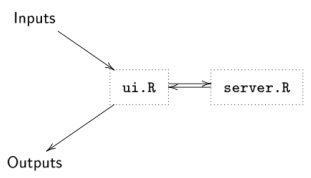
\includegraphics[width=7cm]{./Graficos/figura7}
\end{center}
\caption{Esquema interno de la aplicación.}
\label{fig:fig321}
\end{figure}




\subsection{Flujo de trabajo}

El esta sección se motrará como mejorar dos flujos de trabajo de Shiny importantes: el ciclo de desarrollo básico de crear aplicaciones, realizar cambios y experimentar con los resultados; y la depuración, proceso de identificar y corregir errores de programación.\\


\textbf{1.\hspace{1cm} Flujo de trabajo de desarrollo}\\


El objetivo de optimizar el flujo de trabajo de desarrollo es reducir el tiempo entre hacer un cambio y ver el resultado. Cuanto más rápido se pueda iterar, más rápido se podrá experimentar y más rápido se podrá obtener la Shiny APP. Aquí hay dos flujos de trabajo principales para optimizar: crear la aplicación por primera vez y acelerar el ciclo iterativo de ajustar el código y probar los resultados.\\


\textbf{Creación de la Shiny APP}


Para poder crear una shiny APP se debe tener instado R, RStudio, y el paquete shiny. Una forma de crear la aplicación es crear un nuevo directorio con un sólo archivo llamado app.R. Este archivo especificará la interfaz de usuario así como también las funciones de R que se incluirán.

\begin{lstlisting}
library(shiny)
ui<- ...
server<- ...
shinyApp(ui = ui, server = server)
\end{lstlisting}


Por lo tanto, en el archivo app.R se realizan las siguientes tareas:

\begin{itemize}
\item Carga el paquete shiny: \textcolor{blue}{library}(shiny)
\item Define la interfaz de usuario, la página web HTML con la que los usuarios interactúan.
\item Especifica el comportamiento de la aplicación definiendo la función server. 
\item Se ejecuta función \textcolor{blue}{shinyApp}(ui, server) para construir e iniciar una aplicación Shiny desde la interfaz de usuario y el servidor.
\end{itemize}


La sesión de R estará monitoreando la aplicación y ejecutando las reacciones de la aplicación mientras la aplicación Shiny esté activa, por lo que no se podrá ejecutar ningún comando.

En todo tipo de programación, es una mala práctica tener código duplicado; puede ser un desperdicio computacional y, lo que es más importante, aumenta la dificultad de mantener o depurar el código. En la secuencia de comandos R tradicional, se utilizan dos técnicas para lidiar con el código duplicado: capturar el valor usando una variable o capturar el cálculo con una función. Desafortunadamente, ninguno de estos enfoques funciona en una Shiny APP y se necesita un nuevo mecanismo: expresiones reactivas. Una expresión reactiva tiene una diferencia importante con una variable: sólo se ejecuta la primera vez que se llama y luego almacena en caché el resultado de la misma hasta que necesite actualizarse.

La programación reactiva es un estilo de programación que enfatiza valores que cambian con el tiempo, y cálculos y acciones que dependen de esos valores. Esto es importante para las aplicaciones Shiny porque son interactivas: los usuarios cambian los inputs, lo que hace que la lógica se ejecute en el servidor que finalmente resultan en actualización de los outputs/resultados.\\

\textbf{Ver los cambios}\\

Al crear o modificar la aplicacion, se la ejecuta para poder ver los cambios realizados, por lo que el dominio de flujo de trabajo de desarrollo es especialmente importante. La primera forma de reducir la velocidad de iteración es evitar hacer clic en el botón ``Ejecutar aplicación'' y, en su lugar, aprender el método abreviado de teclado Cmd/Ctrl+ Shift+ Enter. Esto brinda el siguiente flujo de trabajo de desarrollo:

\begin{enumerate}
\item Escribir un código.
\item Iniciar la aplicación con Cmd/Ctrl+ Shift+ Enter.
\item Experimentar interactivamente con la aplicación.
\item Cerrar la aplicación.
\item Ir a 1.
\end{enumerate}


Otra forma de reducir aún más la velocidad de iteración es activar la recarga automática (options(shiny.autoreload = TRUE)) y luego ejecutar la aplicación en un trabajo en segundo plano. Con este flujo de trabajo cuando se guarde un archivo, su aplicación se reiniciará: no es necesario cerrarla y reiniciarla. Esto conduce a un flujo de trabajo aún más rápido:
\begin{enumerate}
\item Escribir un código y presione Cmd/Ctrl+S para guardar en el archivo.
\item Experimentar interactivamente.
\item Ir a 1.
\end{enumerate}
La principal desventaja de esta técnica es que debido a que la aplicación se ejecuta en un proceso separado, es considerablemente más difícil de depurar.


De manera predeterminada, cuando ejecuta la aplicación, aparecerá en una ventana emergente. Sin embargo ,existen otras dos opciones que puede elegir del menú desplegable \emph{Run App}
\begin{enumerate}
\item La ejecución en el panel del visor es útil para aplicaciones más pequeñas porque puede verla al mismo tiempo que ejecuta el código de la aplicación.
\item Ejecutar en un navegador externo es útil para aplicaciones más grandes, o si desea verificar que su aplicación se ve exactamente de la manera que espera en el contexto que la mayoría de los usuarios la verán.
\end{enumerate}


\textbf{2.\hspace{1cm} Depuración}\\


Entre los problemas que pueden surgir al crear una Shiny app se encuentran los siguientes:

\begin{itemize}
\item Error inesperado. Este es el caso más fácil, porque obtendrá un rastreo que le permitirá averiguar exactamente de dónde proviene el error. Una vez que haya identificado el problema, deberá probar sistemáticamente su suposición hasta que encuentre una diferencia entre sus expectativas y lo que realmente está sucediendo. El depurador interactivo es una herramienta poderosa para este proceso.
\item No obtiene ningún error, pero un valor es incorrecto. Aquí, generalmente es mejor transformar esto en el primer problema utilizando stop()para arrojar un error cuando se produce el valor incorrecto.
\item Todos los valores son correctos, pero no se actualizan cuando espera. Este es el problema más desafiante porque es exclusivo de Shiny, por lo que no puede aprovechar sus habilidades de depuración de R.

\end{itemize}


Una vez localizado la fuente del error, la herramienta más poderosa es el depurador interactivo. El depurador detiene la ejecución y le brinda una consola R interactiva donde puede ejecutar cualquier código para descubrir qué salió mal. Hay dos formas de iniciar el depurador:

\begin{itemize}
\item Agregar una llamada a la función browser() en código fuente. Esta es la forma estándar de R de iniciar el depurador interactivo, y funcionará sin embargo, se está ejecutando brillante.
\item Agregar un punto de interrupción RStudio haciendo clic a la izquierda del número de línea. Puede eliminar el punto de interrupción haciendo clic en el círculo rojo. La ventaja de los puntos de interrupción es que no son código, por lo que nunca tendrá que preocuparse por registrarlos accidentalmente en su sistema de control de versiones.
\end{itemize}





\subsection{Compartiendo una Shiny Web App}

Una vez creada la aplicación, resulta conveniente ponerlas a disposición de los usuarios. En este caso la Shiny Web App encuentra disponible en el servidor de CONICET \url{www.cefobi.com}. Además el proyecto se encuentra en GitHub \url{https://github.com/jangelini/shinyAPP_geneticae}. 
